\chapter{Training recipes}


\begin{description}
    \item[Model capacity] \marginnote{Model capacity}
        Capability of a network to fit the train set.
        It depends on the architecture of the model.
    
        \begin{remark}
            By varying the architecture of a model, the resulting network might overfit or underfit.
        \end{remark}

        \begin{figure}[H]
            \centering
            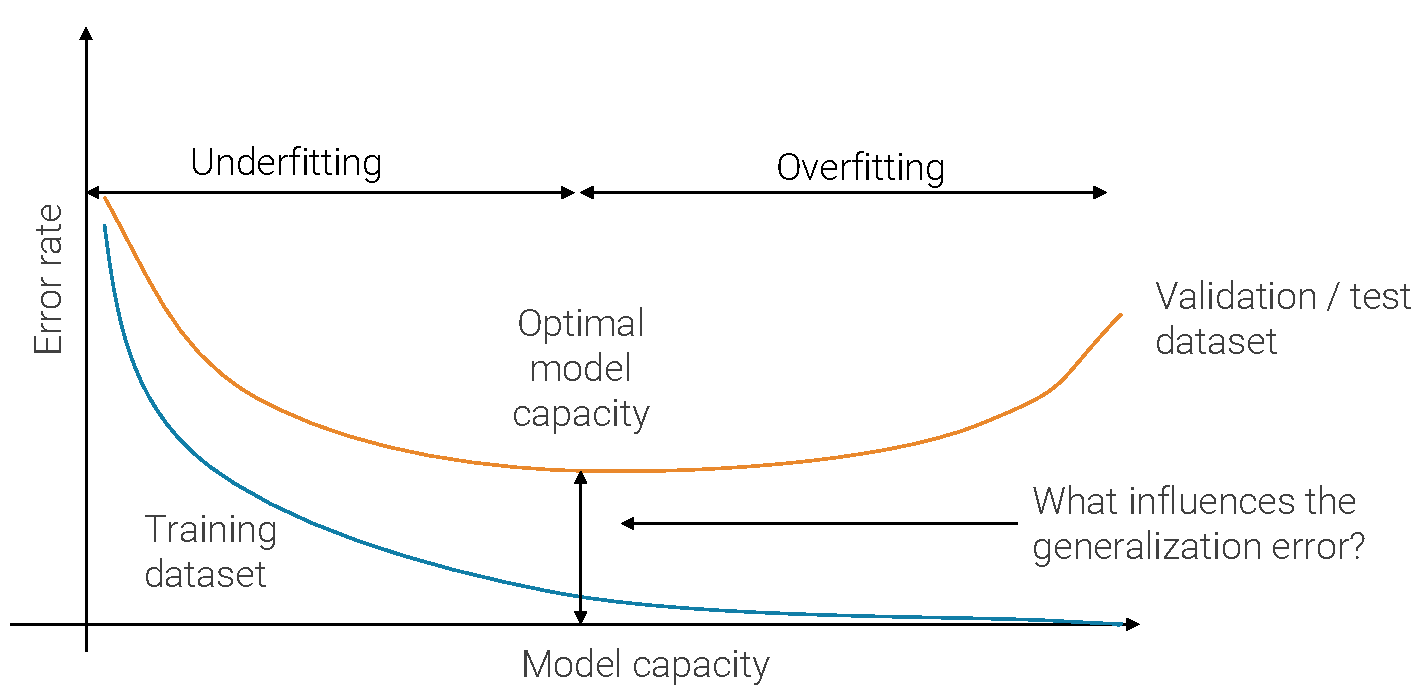
\includegraphics[width=0.6\linewidth]{./img/_model_capacity.pdf}
        \end{figure}


    \item[Effective capacity] \marginnote{Effective capacity}
        Actual capacity of a model that depends on the training hyperparameters (e.g. learning rate, epochs, \dots).

        \begin{remark}
            In practice, a model with a large theoretical capacity is used and it is tuned on its effective capacity.
        \end{remark}
\end{description}



\section{Learning rate schedule}
\marginnote{Learning rate schedule}

Mixture of high and low learning rates to find a good compromise between speed and accuracy.

\begin{remark}
    If the learning rate is too high, after the first iteration, updates might get stuck in a valley.
\end{remark}

\begin{remark}
    Intuitively, learning rate schedulers allow to find wide minima (i.e. skip narrow minima and reach a basin with a minimum more ``compatible'' with the step size).

    Moreover, the optimal loss of the test set is usually a shifted and distorted version of the train loss. Therefore, a wider minimum results in a more robust model.

    \begin{figure}[H]
        \centering
        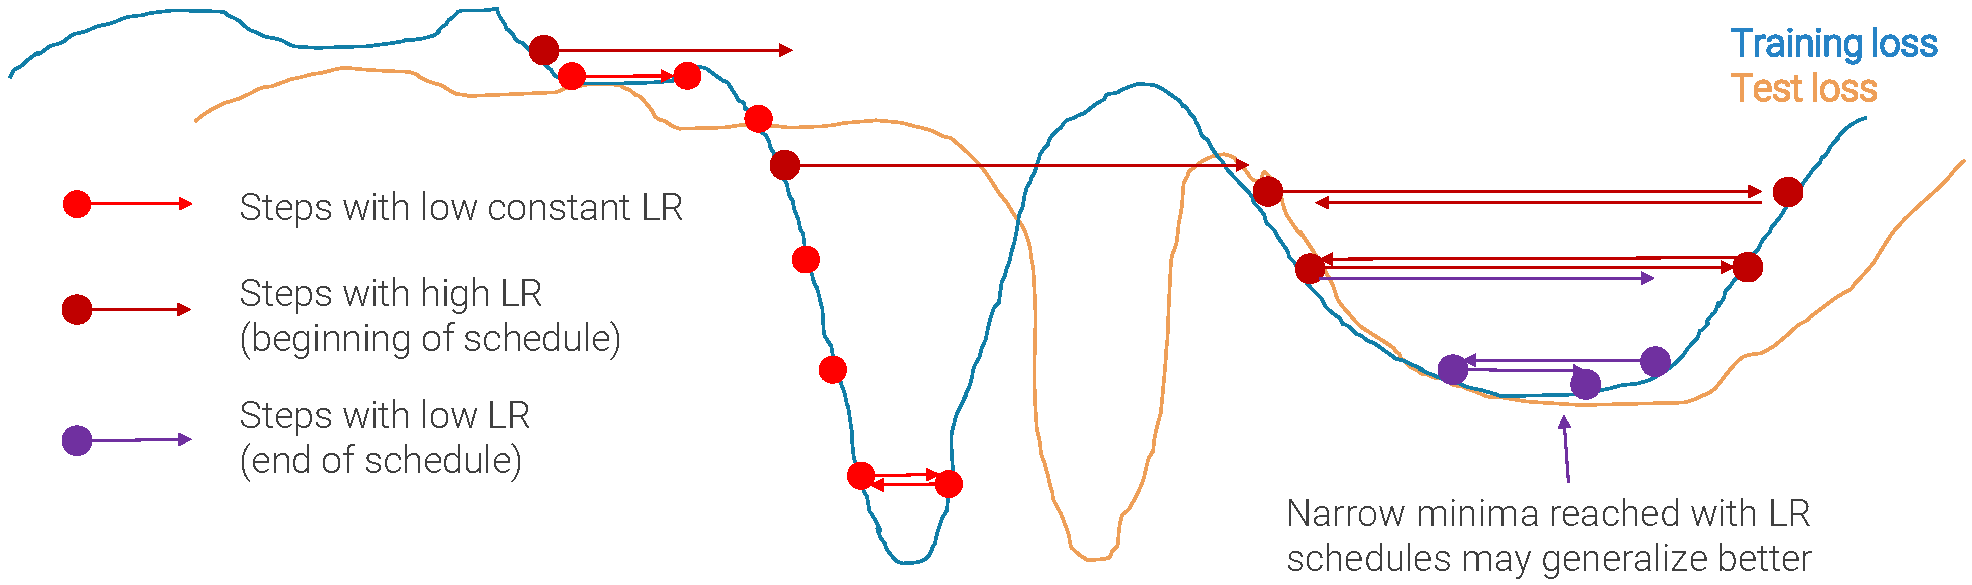
\includegraphics[width=0.9\linewidth]{./img/_lr_schedule_steps.pdf}
    \end{figure}
\end{remark}

\begin{minipage}{0.6\linewidth}
    \begin{description}
        \item[Step]
            Start with a high learning rate and divide it by 10 when reaching a plateau.
    \end{description}
\end{minipage}
\begin{minipage}{0.35\linewidth}
    \begin{figure}[H]
        \centering
        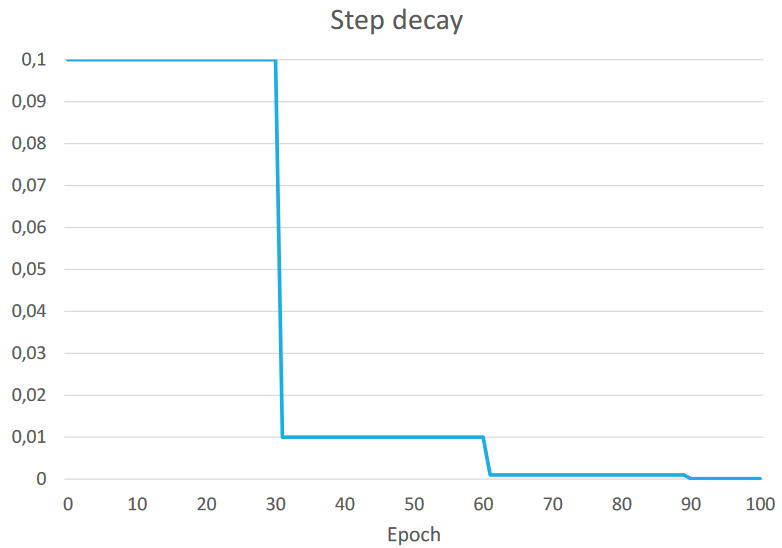
\includegraphics[width=0.9\linewidth]{./img/lr_schedule_step.png}
    \end{figure}
\end{minipage}

\begin{minipage}{0.6\linewidth}
    \begin{description}
        \item[Cosine]
            Continuous decay of the learning rate that follows the cosine function.
            Given the number of training epochs $E$, the starting learning rate $\texttt{lr}_0$ and ending learning rate $\texttt{lr}_E$, the learning rate at epoch $e$ is given by:
            \[ \texttt{lr}_e = \texttt{lr}_E + \frac{1}{2}(\texttt{lr}_0 - \texttt{lr}_E) \left( 1 + \cos\left( \frac{e\pi}{E} \right) \right) \]

            \begin{remark}
                Compared to the step scheduler, it only requires two hyperparameters (starting and ending learning rate).
            \end{remark}
    \end{description}
\end{minipage}
\begin{minipage}{0.35\linewidth}
    \begin{figure}[H]
        \centering
        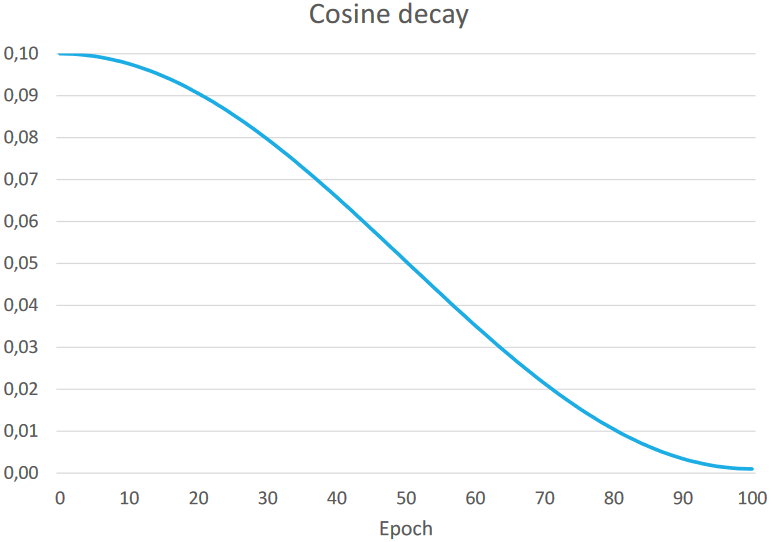
\includegraphics[width=0.9\linewidth]{./img/lr_schedule_cosine.png}
    \end{figure}
\end{minipage}

\begin{minipage}{0.6\linewidth}
    \begin{description}
        \item[Linear]
            Continuous decay of the learning rate that follows a linear function.
            Given the number of training epochs $E$, the starting learning rate $\texttt{lr}_0$ and ending learning rate $\texttt{lr}_E$, the learning rate at epoch $e$ is given by:
            \[ \texttt{lr}_e = \texttt{lr}_E + (\texttt{lr}_0 - \texttt{lr}_E) \left( 1 + \frac{e}{E} \right) \]
    \end{description}
\end{minipage}
\begin{minipage}{0.35\linewidth}
    \begin{figure}[H]
        \centering
        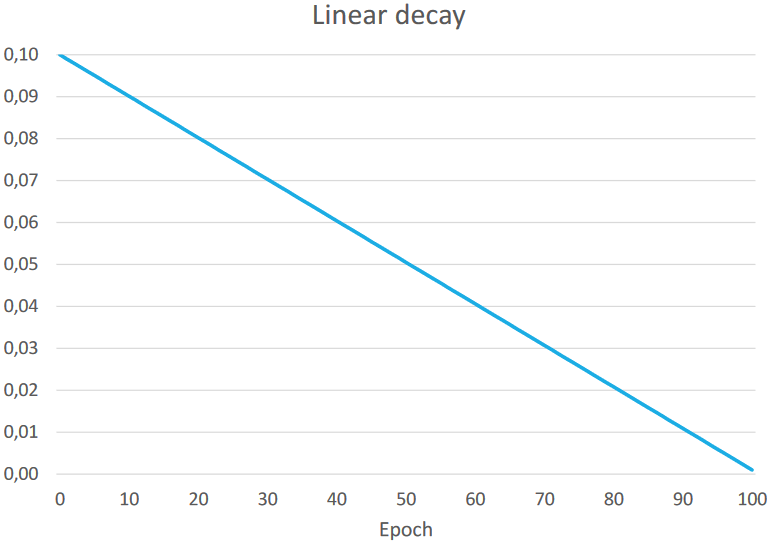
\includegraphics[width=0.9\linewidth]{./img/lr_schedule_linear.png}
    \end{figure}
\end{minipage}

\begin{minipage}{0.6\linewidth}
    \begin{description}
        \item[Warm-up]
            Start with a small learning rate for a few steps (a few epochs or batch steps) before growing and progressively decaying.

            \begin{remark}
                This is useful for large networks where poor initialization and high learning rates at the beginning might slow down convergence.
            \end{remark}
    \end{description}
\end{minipage}
\begin{minipage}{0.35\linewidth}
    \begin{figure}[H]
        \centering
        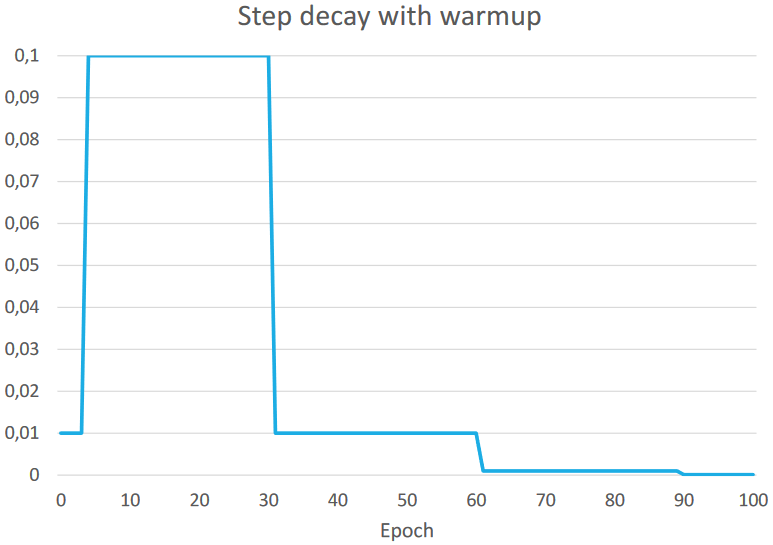
\includegraphics[width=0.9\linewidth]{./img/lr_schedule_warmup.png}
    \end{figure}
\end{minipage}

\begin{description}
    \item[One cycle]
        Scheduler defined on batch steps. It starts with a small learning rate that grows until a maximum is reached after which decay starts.

        \begin{minipage}{0.6\linewidth}
            Given:
            \begin{itemize}
                \item The number of training iterations $I$,
                \item The starting learning rate $\texttt{lr}_0$,
                \item The peak learning rate $\texttt{lr}_{\max}$,
                \item The ending learning rate $\texttt{lr}_{\min}$,
                \item The percentage of iterations $p$ for which the learning rate should increase,
            \end{itemize}
        \end{minipage}
        \begin{minipage}{0.35\linewidth}
            \begin{figure}[H]
                \centering
                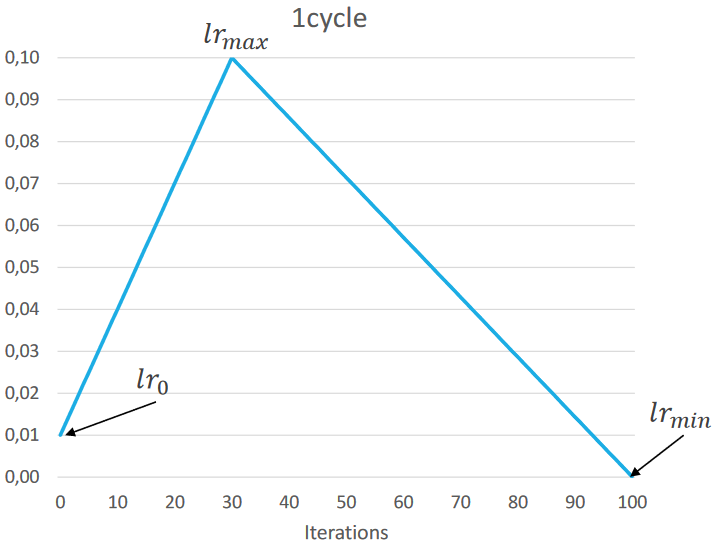
\includegraphics[width=0.9\linewidth]{./img/lr_schedule_1cycle.png}
            \end{figure}
        \end{minipage}

        The learning rate at iteration $i$ is given by:
        \[ 
            \texttt{lr}_i = 
                \begin{cases}
                    \texttt{lr}_{\max} + (\texttt{lr}_0 - \texttt{lr}_{\max}) \left( 1 - \frac{i}{pI} \right) & \text{if $i < pI$} \\
                    \texttt{lr}_{\min} + (\texttt{lr}_0 - \texttt{lr}_{\min}) \left( 1 - \frac{i - pI}{I - pI} \right) & \text{if $i \geq pI$} \\
                \end{cases}
        \]
\end{description}



\section{Regularization}

\begin{description}
    \item[Regularization] \marginnote{Regularization} 
        Modifications to the network that aim to improve its generalization capacity without introducing overfitting.
        \begin{figure}[H]
            \centering
            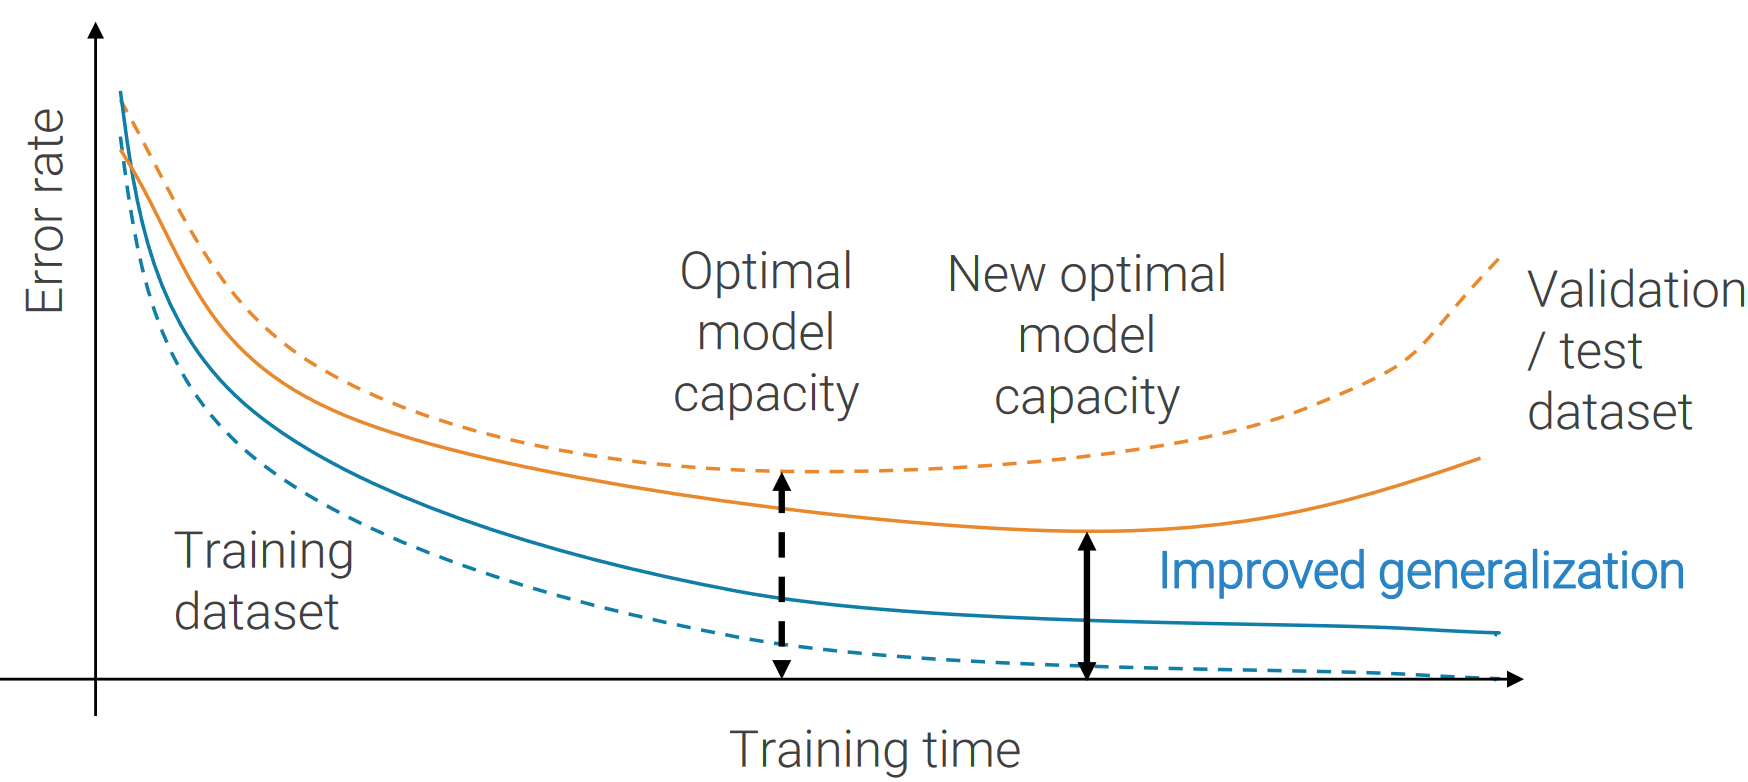
\includegraphics[width=0.5\linewidth]{./img/regularization.png}
        \end{figure}
\end{description}


\subsection{Parameter norm penalties}

Add a regularization term to the loss:
\[ 
    \mathcal{L}(\matr{\theta}; \mathcal{D}^\text{(train)}) = 
        \mathcal{L}^\text{(task)}(\matr{\theta}; \mathcal{D}^\text{(train)}) + 
        \lambda \mathcal{L}^\text{(reg)}(\matr{\theta}) 
\]

\begin{remark}
    Intuitively, normalization forces parameters to be small, therefore, limiting the effective capacity of the model and improving generalization.
\end{remark}

\begin{description}
    \item[L1 regularization] 
        The regularization term is:
        \[ \mathcal{L}^\text{(reg)}(\matr{\theta}) = \sum_{i} \vert \matr{\theta} \vert \]

    \item[L2 regularization] 
        The regularization term is:
        \[ \mathcal{L}^\text{(reg)}(\matr{\theta}) = \sum_{i} \matr{\theta}^2 = \Vert \matr{\theta} \Vert_2^2 \]

        \begin{remark}
            When using plain SGD, L2 regularization is also called weight decay.
            In fact, given the loss:
            \[ 
                \mathcal{L}(\matr{\theta}; \mathcal{D}^\text{(train)}) = 
                \mathcal{L}^\text{(task)}(\matr{\theta}; \mathcal{D}^\text{(train)}) + 
                \frac{\lambda}{2} \Vert \matr{\theta} \Vert_2^2
            \]
            The gradient update is:
            \[
                \begin{split}
                    \matr{\theta}^{(i+1)} &= \matr{\theta}^{(i)} - \texttt{lr} \nabla_\matr{\theta} \mathcal{L}(\matr{\theta}^{(i)}; \mathcal{D}^\text{(train)}) \\
                        &= \matr{\theta}^{(i)} - \texttt{lr} \nabla_\matr{\theta}\left[ 
                                \mathcal{L}^\text{(task)}(\matr{\theta}; \mathcal{D}^\text{(train)}) + 
                                \frac{\lambda}{2} \Vert \matr{\theta}^{(i)} \Vert_2^2
                            \right] \\
                        &= \matr{\theta}^{(i)} - \texttt{lr} \left[ 
                                \nabla_\matr{\theta} \mathcal{L}^\text{(task)}(\matr{\theta}; \mathcal{D}^\text{(train)}) + 
                                \lambda \matr{\theta}^{(i)}
                            \right] \\
                        &= 
                            \underbrace{(1 - \texttt{lr} \lambda) \matr{\theta}^{(i)}}_{\mathclap{\text{Decayed parameter vector \phantom{aaaa}}}} - 
                            \underbrace{\texttt{lr} \nabla_\matr{\theta} \mathcal{L}^\text{(task)}(\matr{\theta}; \mathcal{D}^\text{(train)})}_{\mathclap{\text{\phantom{aaaa} Standard gradient descent step}}}
                \end{split}  
            \]
        \end{remark}

        \begin{remark}
            The \texttt{weight\_decay} of more advanced optimizers (e.g. Adam) is not always the L2 regularization.
            
            In PyTorch, \texttt{Adam} implements L2 regularization while \texttt{AdamW} uses another type of regularizer.
        \end{remark}
\end{description}


\subsection{Early stopping}
\marginnote{Early stopping}

Monitor performance on the validation set and either:
\begin{itemize}
    \item Select the checkpoint with the best validation set after a maximum number of epochs.
    \item Set a hyperparameter (patience) that stops training if, after a certain number of steps, validation performance does not improve.
\end{itemize}

\begin{remark}
    If possible, the first option is preferable as validation metrics might improve after a few steps of stagnation or decrease.
\end{remark}


\subsection{Label smoothing}
\marginnote{Label smoothing}

When using cross-entropy with softmax, the model has to push the correct logit to $+\infty$ and the others to $-\infty$ so that the softmax outputs $1$ for the correct label. This is unnecessary as it might cause overfitting.

Given $C$ classes, labels can be smoothed by assuming a small uniform noise $\varepsilon$:
\[
    \vec{y}^{(i)} = \begin{cases}
        1 - \frac{\varepsilon(C-1)}{C} & \text{if $i$ is the correct label} \\
        \frac{\varepsilon}{C} & \text{otherwise} \\
    \end{cases}
\]


\subsection{Dropout}

\begin{description}
    \item[Train time] \marginnote{Dropout}
        For each batch step, generate a mask that sets some activations (usually $10\% - 50\%$) to zero during the forward pass.
        
        \begin{remark}
            Intuitively, activations that are not dropped should learn to not rely on the other neurons and therefore avoiding focusing on selective information.
        \end{remark}
        
        \begin{remark}
            Dropout can be seen as an ensemble of models where each mask is a new model.
        \end{remark}

    \item[Test time] 
        With dropout, the output of the network is non-deterministic and methods to make inference more deterministic should be applied:
        \begin{description}
            \item[Naive approach] 
                A naive workaround is to sample some random masks and average the outputs of the network on these masks:
                \[ f(\vec{x}; \matr{\theta}) = \mathbb{E}_\matr{m} [ f(\vec{x}; \matr{\theta}, \matr{m}) ] = \sum_\matr{m} p(\matr{m}) f(\vec{x}; \matr{\theta}, \matr{m}) \]
                Although more accurate, this method is computationally expensive.

            \item[Weight scaling] 
                Without loss of generality, consider an activation $a$ obtained as a linear combination of two neurons $x_1$ and $x_2$.
                During test time, the activation is:
                \[ a^\text{(test)} = w_1 x_1 + w_2 x_2 \]
                Assuming a dropout with $p=0.5$ (a neuron has a $50\%$ probability of being dropped), the expected value of the activation $a^\text{(train)}$ at train time is:
                \[  
                    \begin{split}
                        \mathbb{E}_\matr{m} [ a^\text{(train)} ] &= \frac{1}{4}(w_1 x_1 + w_2 x_2) + \frac{1}{4}(w_1 x_1 + 0) + \frac{1}{4}(0 + w_2 x_2) + \frac{1}{4}(0 + 0) \\
                            &= \frac{1}{2}(w_1 x_1 + w_2 x_2) = p a^\text{(test)}
                    \end{split}
                \]
                There is, therefore, a $p$ factor of discrepancy between $a^\text{(train)}$ and $a^\text{(test)}$ that might disrupt the distribution of the activations. Two approaches can be taken:
                \begin{itemize}
                    \item Rescale the value at test time:
                        \[ p a^\text{(test)} = \mathbb{E}_\matr{m} \left[ a^\text{(train)} \right] \]

                    \item Rescale the value at train time (inverted dropout):
                        \[ a^\text{(test)} = \mathbb{E}_\matr{m} \left[ \frac{a^\text{(train)}}{p} \right] \]
                        This approach is preferred as it leaves test time unchanged.
                \end{itemize}

                \begin{remark}
                    Weight scaling is exact only for linear layers. Still, with a non-linear activation, this method is a fast approximation of the output of the network with dropout.
                \end{remark}
        \end{description}
\end{description}

\begin{remark}
    Dropout on convolutional layers are usually not necessary as they already have a strong inductive bias.
\end{remark}

\begin{remark}
    Dropout and batch normalization show a general pattern for regularization:
    \begin{itemize}
        \item At train time, some randomness is added.
        \item At test time, inference is done by averaging or approximating the output of the network.
    \end{itemize}
\end{remark}


\subsection{Data augmentation}
\marginnote{Data augmentation}

Increase the size of a dataset by manipulating (e.g. flipping) the existing examples.

\begin{remark}
    More data always reduces variance and is therefore always a positive thing.
\end{remark}

\begin{remark}
    Transformations should be label-preserving (e.g. a $180^\circ$ rotation should not be applied on a $6$ or $9$).
\end{remark}


\begin{description}
    \item[Multi-scale training] \marginnote{Multi-scale training}
        Sample random crops and scales:

        \begin{minipage}{0.7\linewidth}
            \begin{enumerate}
                \item Choose a random size $S$ in range $[S_{\min}, S_{\max}]$.
                \item Isotropically (i.e. preserve the aspect ratio) scale the training image so that the short side is of size $S$.
                \item Sample random patches of a given size.
            \end{enumerate}
        \end{minipage}
        \begin{minipage}{0.2\linewidth}
            \begin{figure}[H]
                \centering
                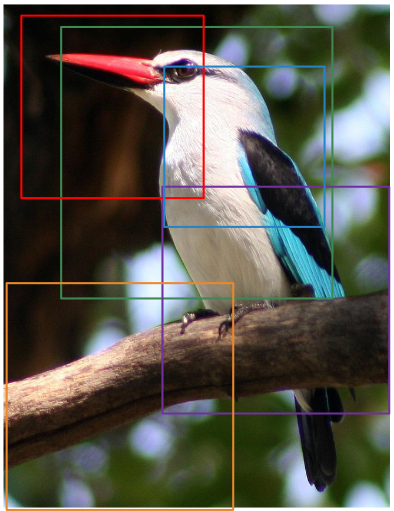
\includegraphics[width=0.9\linewidth]{./img/multi_scale_augmentation.png}
            \end{figure}
        \end{minipage}

        \begin{remark}
            For $S$ close to the patch size, crops will capture whole-image statistics.
            For $S$ bigger than the patch size, crops will cover small portions of the image (with the risk of getting areas where the target content is not present).
        \end{remark}

    \item[FixRes] \marginnote{FixRes}
        At test time, the image is usually presented with the target at the center (photographer bias) at a specific size. 
        However, using data augmentation at train time, the size of the crops of the target varies following a distribution that is different from the one of the test set and usually involves smaller crops of the input image.

        \begin{figure}[H]
            \centering
            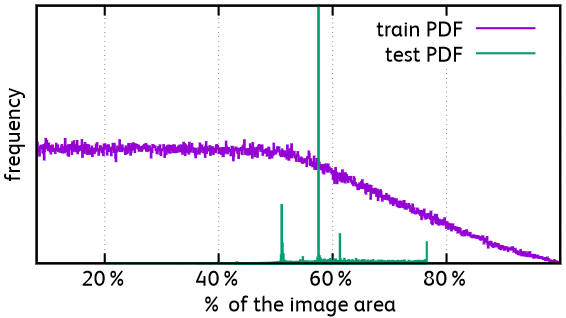
\includegraphics[width=0.35\linewidth]{./img/fixres1.png}
        \end{figure}

        Therefore, there is a discrepancy between train and test images as, during training, the network sees objects that are bigger due to the rescaling of the input image.

        It has been shown that a possible solution to close this discrepancy is to train the model using images with a lower resolution than the test set. The possible alternatives are:
        \begin{itemize}
            \item Reduce train-time resolution.
            \item Reduce test-time resolution.
        \end{itemize}
        \begin{figure}[H]
            \centering
            \begin{subfigure}{0.6\linewidth}
                \centering
                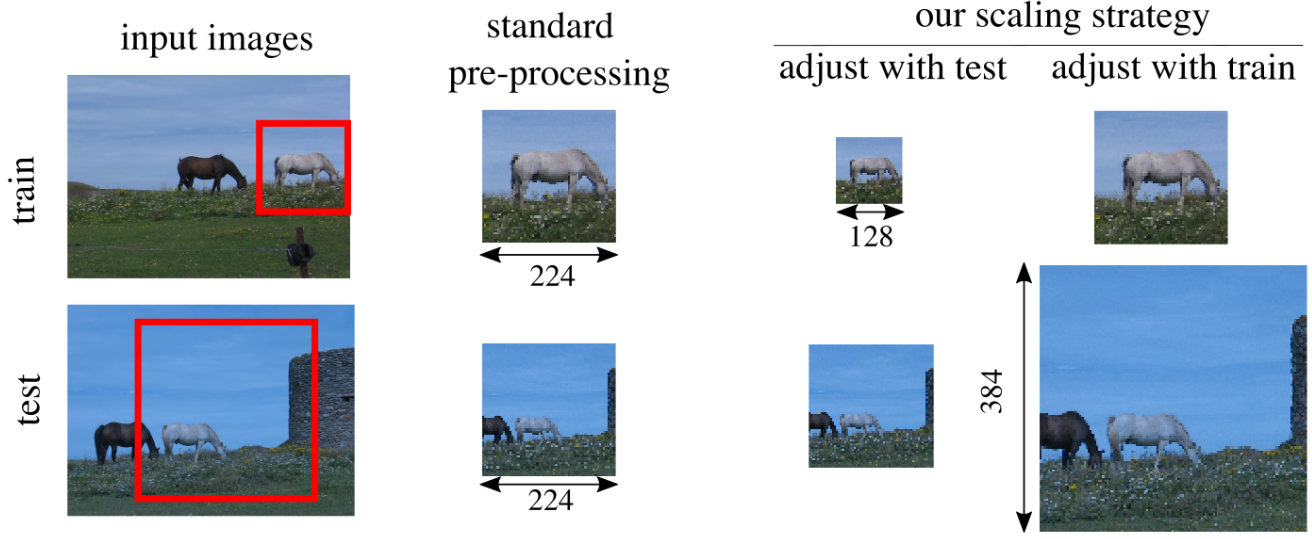
\includegraphics[width=0.9\linewidth]{./img/fixres2.png}
            \end{subfigure}
            \begin{subfigure}{0.38\linewidth}
                \centering
                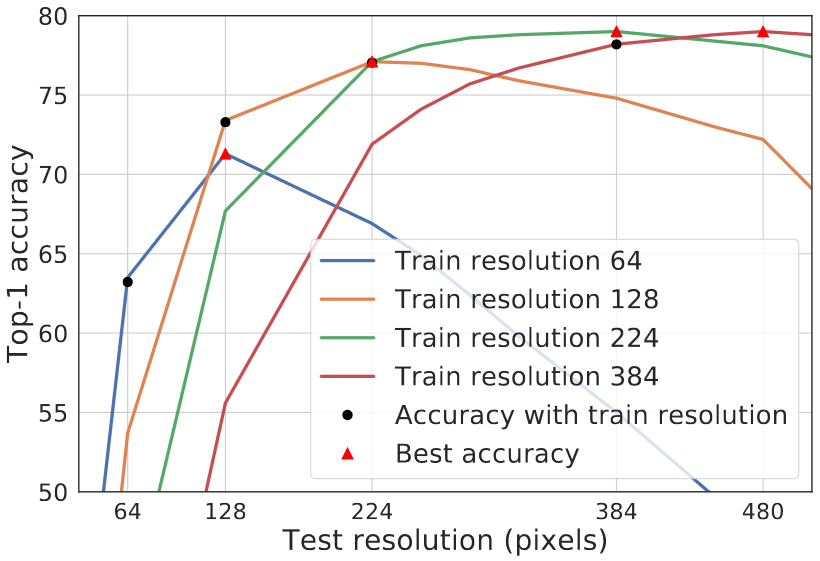
\includegraphics[width=0.9\linewidth]{./img/fixres3.png}
            \end{subfigure}
        \end{figure}
\end{description}